\pdfbookmark{Общая характеристика работы}{characteristic}             % Закладка pdf
\section*{Общая характеристика работы}

\newcommand{\actuality}{\pdfbookmark[1]{Актуальность}{actuality}\underline{\textbf{\actualityTXT}}}
\newcommand{\progress}{\pdfbookmark[1]{Разработанность темы}{progress}\underline{\textbf{\progressTXT}}}
\newcommand{\aim}{\pdfbookmark[1]{Цели}{aim}\underline{{\textbf\aimTXT}}}
\newcommand{\tasks}{\pdfbookmark[1]{Задачи}{tasks}\underline{\textbf{\tasksTXT}}}
\newcommand{\aimtasks}{\pdfbookmark[1]{Цели и задачи}{aimtasks}\aimtasksTXT}
\newcommand{\novelty}{\pdfbookmark[1]{Научная новизна}{novelty}\underline{\textbf{\noveltyTXT}}}
\newcommand{\influence}{\pdfbookmark[1]{Практическая значимость}{influence}\underline{\textbf{\influenceTXT}}}
\newcommand{\methods}{\pdfbookmark[1]{Методология и методы исследования}{methods}\underline{\textbf{\methodsTXT}}}
\newcommand{\defpositions}{\pdfbookmark[1]{Положения, выносимые на защиту}{defpositions}\underline{\textbf{\defpositionsTXT}}}
\newcommand{\reliability}{\pdfbookmark[1]{Достоверность}{reliability}\underline{\textbf{\reliabilityTXT}}}
\newcommand{\probation}{\pdfbookmark[1]{Апробация}{probation}\underline{\textbf{\probationTXT}}}
\newcommand{\contribution}{\pdfbookmark[1]{Личный вклад}{contribution}\underline{\textbf{\contributionTXT}}}
\newcommand{\publications}{\pdfbookmark[1]{Публикации}{publications}\underline{\textbf{\publicationsTXT}}}


{\actuality} В современном мире, где преобладают мобильные системы, роль серверных вычислений постоянно возрастает. В период с 2013 до 2023 год объем денежных средств, вкладываемых  международными компаниями в облачные вычисления увеличился в 5 раз \cite{spendingCloud,alam2020cloud} и достиг сотни миллиардов долларов США. Многие современные приложения не могут быть запущены на мобильных и домашних устройствах в силу огромного количества потребляемых ресурсов \cite{marinescu2022cloud}.
Сегодня цена вычислительных мощностей варьируется от 60 до 1500  долларов в месяц за единицу \cite{costCloud}.  У одной только российской компании Яндекс на сегодняшний день имеется от 150 000  до 200 000 серверов в 5 датацентрах по всему миру \cite{Yndx2}. Соответственно вопрос производительности программного обеспечения на серверах стоит достаточно остро.

Из года в год различные вендоры вычислительной техники соревнуются в производительности своей продукции. Основными компонентами производительности процессора являются IPC (количество инструкций, исполняемы за один машинный такт), частота и количество выполненных инструкций \cite{hennessy2011computer}. Со стороны компилятора можно повлиять на количество инструкций и лучше использовать возможности оборудования, чтобы увеличить IPC \cite{alvares2021instruction}.

$$performance = IPC * \dfrac{frequency}{executed\_instructions}$$

GCC (GNU Compiler Colection) — это хорошо известный компилятор \cite{schmitt2020performance}, который содержит десятки различных архитектурно-зависимых и независимых от архитектуры оптимизаций \cite {rodriguez2021compiler}. Имеет открытый исходный код и ориентирован на оптимизацию C, C++ и Fortran.

Настройка компилятора для конкретной архитектуры или набора тестов — это необходимая работа, которая помогает компании продемонстрировать наилучшую производительность. Например, Дмитрий Мельник и др. all \cite{melnik2010case} оптимизировали GCC для библиотеки растеризации libevas, продемонстрировав, что GCC имеет недостатки в алгоритме распределения регистров для ARM. Кроме того,в этой же работе был проведен анализ различных типов предварительной выборки данных. Многие другие авторы предлагали методы автоматической конфигурации или настройки компилятора \cite{plotnikov2013automatic,ashouri2018survey,cereda2020collaborative}. Однако данная работа была сосредоточена не на настройке существующих оптимизаций, а на их усовершенствовании и разработке новых.


В настоящее время большинство компаний используют SPEC CPU 2017 для измерения производительности компьютера \cite{panda2018wait,bucek2018spec}. Недавно был представлен новый инструмент оценки производительности под названием CPUBench \cite {lu2023cpubench}. В ходе исследования выяснилось, что GCC очень хорошо настроен для SPEC CPU 2017, в то время как для другого набора тестов (CPUBench) все еще остается много возможностей для улучшения.

%\ifsynopsis
%Этот абзац появляется только в~автореферате.
%Для формирования блоков, которые будут обрабатываться только в~автореферате,
%аведена проверка условия \verb!\!\verb!ifsynopsis!.
%Значение условия задаётся в~основном файле документа (\verb!synopsis.tex! для
%автореферата).
%\else
%Этот абзац появляется только в~диссертации.
%Через проверку условия \verb!\!\verb!ifsynopsis!, задаваемого в~основном файле
%документа (\verb!dissertation.tex! для диссертации), можно сделать новую
%команду, обеспечивающую появление цитаты в~диссертации, но~не~в~автореферате.
%\fi

% {\progress}
% Этот раздел должен быть отдельным структурным элементом по
% ГОСТ, но он, как правило, включается в описание актуальности
% темы. Нужен он отдельным структурынм элемементом или нет ---
% смотрите другие диссертации вашего совета, скорее всего не нужен.

{\aim} данной работы является 
разработка новой версии компилятора GCC, ориентированного на микроархитектуру китайского производителя кристалла, основанного на архитектуре АРМV8-64, 
и компьютера целиком.
Для~достижения поставленной цели необходимо было решить следующие {\tasks}:
\begin{enumerate}[beginpenalty=10000] % https://tex.stackexchange.com/a/476052/104425
  \item Исследовать текущую производительность  компилятора GCC в смысле тестовых пакетов CPUbench и SPEC 2017. 
  \item Выяснить слабые места анализируемой микроархитектуры c помощью моделей и экспериментов.
  \item Исследовать похожие проблемы в научной литературе и предложить решение, позволяющее увеличить производительность целевых приложений.
  \item Исследовать код целевого набора приложений на предмет неоптимальностей с точки зрения целевой микроархитектуры.
  \item Разработать продуктовое решение в компиляторе GCC, позволяющее получить ускорение на целевых тестах компании.
  \item Протестировать разработанные методы на реальных приложениях. 
\end{enumerate}

Тема и содержание диссертационной работы соответствует паспорту научной
специальности 2.3.5 – Математическое и программное обеспечение
6
вычислительных машин, комплексов и компьютерных сетей, в частности, пунктам:

п. 1 – Модели, методы и алгоритмы проектирования и анализа программ
и программных систем, их эквивалентных преобразований, верификации и тестирования.

п. 3 – Модели, методы, алгоритмы, языки и программные инструменты
для организации взаимодействия программ и программных систем.

{\novelty}
\begin{enumerate}[beginpenalty=10000] % https://tex.stackexchange.com/a/476052/104425
  \item Было выполнено оригинальное исследование производительности целевой микроархитектуры.
  \item Было разработано и имплементировано в продукт более десяти различных оптимизаций в компиляторе GCC.
  \item Впервые была исследована проблема производительности широких инструкций доступа в память и предложена оптимизация, разрешающая ее. 
  \item Впервые был представлен алгоритм автоматического подбора вероятностей условных переходов для компилятора GCC.
\end{enumerate}

{\influence}  данной работы заключается в использовании
разработанных методов и алгоритмов в  компиляторе с открытым исходным кодом  ООО «Техкомпания Хуавэй
»  openEuler GCC и его
инфраструктуре для оптимизации приложений и последующем использовании пользователями. Реализованные оптимизации, верификации
и методы получения профильной информации позволили получить прирост производительности
на целевых приложениях компании.

Теоретическая значимость диссертационной работы заключается в разработке
новых алгоритмов и методов микроархитектурных оптимизаций, позволяющих раскрыть потенциал производительности целевой архитектуры.

{\defpositions}
\begin{enumerate}[beginpenalty=10000] % https://tex.stackexchange.com/a/476052/104425
  \item Улучшение алгоритма преобразования условных переходов.
  \item Алгоритм шаблонной оптимизации двойного умножения.
  \item Алгоритм разбиения широких инструкций доступа в память.
  \item Алгоритм слияния "хвостов" базовых блоков.
  \item Алгоритм векторизации ленивых вычислений.
  \item Алгоритм автоматического подбора вероятностей условных переходов.
\end{enumerate}

{\reliability} полученных результатов и выводов обеспечивается подробным описанием проведенных экспериментом, а также возможностью их повторения. Результаты находятся в соответствии с результатами, полученными другими авторами.


{\probation}
Основные результаты работы докладывались~на:
\begin{enumerate}[beginpenalty=10000] % https://tex.stackexchange.com/a/476052/104425
	\item 63-й всероссийской научной конференции московского физико–
	технического института (государственного университета), Москва,
	ноябрь 2020 г.
	\item 66-й всероссийской научной конференции московского физико–
	технического института (государственного университета), Москва,
	ноябрь 2024 г.
	\item 4-й Международной конференции о достижениях вычислительных технологий и искусственного интеллекта, Касабланка, 2024 г.
\end{enumerate}

{\contribution} В течение нескольких лет автор данной диссертации являлся техническим руководителем команды из 10 человек по разработке openEuler GCC в России. В течение этого времени и были разработаны представленные в данной работе алгоритмы и оптимизации. Часть из них, такие как  улучшение преобразования условных переходов или векторизация циклов с малым числом итераций  были разработаны автором полностью самостоятельно. Некоторые оптимизации, такие как векторизация ленивых вычислений, разбиение широких инструкций доступа в память, автоматический подбор вероятностей условных переходов и др., были разработаны студентами, находящимися под непосредственным руководством автора данной диссертации. Отдельные оптимизации были разработаны инженерами, находящимися под технических руководством автора.
\ifnumequal{\value{bibliosel}}{0}
{%%% Встроенная реализация с загрузкой файла через движок bibtex8. (При желании, внутри можно использовать обычные ссылки, наподобие `\cite{vakbib1,vakbib2}`).
    {\publications} Основные результаты по теме диссертации изложены
    в~XX~печатных изданиях,
    X из которых изданы в журналах, рекомендованных ВАК,
    X "--- в тезисах докладов.
}%
{%%% Реализация пакетом biblatex через движок biber
    \begin{refsection}[bl-author, bl-registered]
        % Это refsection=1.
        % Процитированные здесь работы:
        %  * подсчитываются, для автоматического составления фразы "Основные результаты ..."
        %  * попадают в авторскую библиографию, при usefootcite==0 и стиле `\insertbiblioauthor` или `\insertbiblioauthorgrouped`
        %  * нумеруются там в зависимости от порядка команд `\printbibliography` в этом разделе.
        %  * при использовании `\insertbiblioauthorgrouped`, порядок команд `\printbibliography` в нём должен быть тем же (см. biblio/biblatex.tex)
        %
        % Невидимый библиографический список для подсчёта количества публикаций:
        \printbibliography[heading=nobibheading, section=1, env=countauthorvak,          keyword=biblioauthorvak]%
        \printbibliography[heading=nobibheading, section=1, env=countauthorwos,          keyword=biblioauthorwos]%
        \printbibliography[heading=nobibheading, section=1, env=countauthorscopus,       keyword=biblioauthorscopus]%
        \printbibliography[heading=nobibheading, section=1, env=countauthorconf,         keyword=biblioauthorconf]%
        \printbibliography[heading=nobibheading, section=1, env=countauthorother,        keyword=biblioauthorother]%
        \printbibliography[heading=nobibheading, section=1, env=countregistered,         keyword=biblioregistered]%
        \printbibliography[heading=nobibheading, section=1, env=countauthorpatent,       keyword=biblioauthorpatent]%
        \printbibliography[heading=nobibheading, section=1, env=countauthorprogram,      keyword=biblioauthorprogram]%
        \printbibliography[heading=nobibheading, section=1, env=countauthor,             keyword=biblioauthor]%
        \printbibliography[heading=nobibheading, section=1, env=countauthorvakscopuswos, filter=vakscopuswos]%
        \printbibliography[heading=nobibheading, section=1, env=countauthorscopuswos,    filter=scopuswos]%
        %
        \nocite{*}%
        %
        {\publications} Основные результаты по теме диссертации изложены в~\arabic{citeauthor}~печатных изданиях,
        \arabic{citeauthorvak} из которых изданы в журналах, рекомендованных ВАК\sloppy%
        \ifnum \value{citeauthorscopuswos}>0%
            , \arabic{citeauthorscopuswos} "--- в~периодических научных журналах, индексируемых Web of~Science и Scopus\sloppy%
        \fi%
        \ifnum \value{citeauthorconf}>0%
            , \arabic{citeauthorconf} "--- в~тезисах докладов.
        \else%
            .
        \fi%
        \ifnum \value{citeregistered}=1%
            \ifnum \value{citeauthorpatent}=1%
                Зарегистрирован \arabic{citeauthorpatent} патент.
            \fi%
            \ifnum \value{citeauthorprogram}=1%
                Зарегистрирована \arabic{citeauthorprogram} программа для ЭВМ.
            \fi%
        \fi%
        \ifnum \value{citeregistered}>1%
            Зарегистрированы\ %
            \ifnum \value{citeauthorpatent}>0%
            \formbytotal{citeauthorpatent}{патент}{}{а}{}\sloppy%
            \ifnum \value{citeauthorprogram}=0 . \else \ и~\fi%
            \fi%
            \ifnum \value{citeauthorprogram}>0%
            \formbytotal{citeauthorprogram}{программ}{а}{ы}{} для ЭВМ.
            \fi%
        \fi%
        % К публикациям, в которых излагаются основные научные результаты диссертации на соискание учёной
        % степени, в рецензируемых изданиях приравниваются патенты на изобретения, патенты (свидетельства) на
        % полезную модель, патенты на промышленный образец, патенты на селекционные достижения, свидетельства
        % на программу для электронных вычислительных машин, базу данных, топологию интегральных микросхем,
        % зарегистрированные в установленном порядке.(в ред. Постановления Правительства РФ от 21.04.2016 N 335)
    \end{refsection}%
    \begin{refsection}[bl-author, bl-registered]
        % Это refsection=2.
        % Процитированные здесь работы:
        %  * попадают в авторскую библиографию, при usefootcite==0 и стиле `\insertbiblioauthorimportant`.
        %  * ни на что не влияют в противном случае
        \nocite{vakbib2}%vak
        \nocite{patbib1}%patent
        \nocite{progbib1}%program
        \nocite{bib1}%other
        \nocite{confbib1}%conf
    \end{refsection}%
        %
        % Всё, что вне этих двух refsection, это refsection=0,
        %  * для диссертации - это нормальные ссылки, попадающие в обычную библиографию
        %  * для автореферата:
        %     * при usefootcite==0, ссылка корректно сработает только для источника из `external.bib`. Для своих работ --- напечатает "[0]" (и даже Warning не вылезет).
        %     * при usefootcite==1, ссылка сработает нормально. В авторской библиографии будут только процитированные в refsection=0 работы.
}

%При использовании пакета \verb!biblatex! будут подсчитаны все работы, добавленные
%в файл \verb!biblio/author.bib!. Для правильного подсчёта работ в~различных
%системах цитирования требуется использовать поля:
%\begin{itemize}
%        \item \texttt{authorvak} если публикация индексирована ВАК,
%        \item \texttt{authorscopus} если публикация индексирована Scopus,
%        \item \texttt{authorwos} если публикация индексирована Web of Science,
%        \item \texttt{authorconf} для докладов конференций,
%        \item \texttt{authorpatent} для патентов,
%        \item \texttt{authorprogram} для зарегистрированных программ для ЭВМ,
%        \item \texttt{authorother} для других публикаций.
%\end{itemize}
%Для подсчёта используются счётчики:
%\begin{itemize}
%        \item \texttt{citeauthorvak} для работ, индексируемых ВАК,
%        \item \texttt{citeauthorscopus} для работ, индексируемых Scopus,
%        \item \texttt{citeauthorwos} для работ, индексируемых Web of Science,
%        \item \texttt{citeauthorvakscopuswos} для работ, индексируемых одной из трёх баз,
%        \item \texttt{citeauthorscopuswos} для работ, индексируемых Scopus или Web of~Science,
%        \item \texttt{citeauthorconf} для докладов на конференциях,
%        \item \texttt{citeauthorother} для остальных работ,
%        \item \texttt{citeauthorpatent} для патентов,
%        \item \texttt{citeauthorprogram} для зарегистрированных программ для ЭВМ,
%        \item \texttt{citeauthor} для суммарного количества работ.
%\end{itemize}
% Счётчик \texttt{citeexternal} используется для подсчёта процитированных публикаций;
% \texttt{citeregistered} "--- для подсчёта суммарного количества патентов и программ для ЭВМ.

%Для добавления в список публикаций автора работ, которые не были процитированы в
%автореферате, требуется их~перечислить с использованием команды \verb!\nocite! в
%\verb!Synopsis/content.tex!.
 % Характеристика работы по структуре во введении и в автореферате не отличается (ГОСТ Р 7.0.11, пункты 5.3.1 и 9.2.1), потому её загружаем из одного и того же внешнего файла, предварительно задав форму выделения некоторым параметрам

%Диссертационная работа была выполнена при поддержке грантов \dots

%\underline{\textbf{Объем и структура работы.}} Диссертация состоит из~введения,
%четырех глав, заключения и~приложения. Полный объем диссертации
%\textbf{ХХХ}~страниц текста с~\textbf{ХХ}~рисунками и~5~таблицами. Список
%литературы содержит \textbf{ХХX}~наименование.

\pdfbookmark{Содержание работы}{description}                          % Закладка pdf
\section*{Содержание работы}

Во \underline{\textbf{введении}} обосновывается актуальность исследований, проводимых в рамках данной диссертационной работы, приводится обзор научной литературы по изучаемой проблеме, формулируется цель, ставятся задачи, излагается научная новизна и практическая значимость представленного исследования. В последующих главах сначала производится обзор существующих решений по данной тематике, затем описывается методология получения новых оптимизаций а также принципы и сложности замера итоговой производительности. В последней главе описаны алгоритмы, которые позволили улучшить производительность приложений и преодолеть недостатки целовой архитектуры.


\underline{\textbf{Первая глава}} посвящена обзору существующих алгоритмов оптимизации
для ARM64 и других подобных RISC-архитектур. Классические и известные
компиляторные оптимизации (такие как удаление мертвого кода, поиск общих
подвыражений, ленивое перемещение кода и подобные) не описываются в данной работе и считаются общеизвестными, однако могут быть описаны их модификации, которые
позволяют получить улучшение производительности для архитектуры ARM64.
GCC является одним из наиболее известных статических трансляторов
кода. Количество оптимизирующих проходов этого компилятора исчисляется
сотнями, и, тем не менее, его улучшение происходит до сих пор, и каждый
год обнаруживаются новые возможности для оптимизации даже в классических
проходах. 




\underline{\textbf{В разделе 1.1}} приводится описание методологии распределения регистров
и ее современные улучшения. Распределение регистров наравне с выбором и расстановкой инструкций
является одной из самых сложных оптимизаций в компиляторе. В  основе распределения регистров лежит проблема ограниченности размера
регистрового файла аппаратуры. Компилятор внутри себя чаще всего
использует так называемые виртуальные регистры, количество которых неограниченно,
и компилятор не заботится об их переиспользовании. Существуют два базовых алгоритма решения данной задачи: раскраска графа и линейное сканирование. Алгоритм раскараски графа чаще всего дает лучшее решение, однако, когда речь идет о системах, к которым выдвигаются требования
высокой производительности, например, бинарная трансляция, то часто используется
метод линейного санирования. Рассматривается  оптимизация, в которой вводится понятие "активная в
будущем" переменная - переменная, которая будет использоваться инструкциями
при дальнейшем сканировании. Это позволило добиться того, что для 90 \%
инструкций и 80 \% методов модель анализа интервалов жизни стала ненужной. Другая рассмотренная работа показывает, что современный рассматриваемый в работе компилятор все еще может генерировать лишние инструкции загрузки из памяти в
следствие неточности округлений, связанных с использованием целочисленных
вероятностей в компиляторе GCC.

\underline{\textbf{В разделе 1.2}}  рассматривается оптимизация векторизации, развитие которой
тесно связано с развитием современных векторных архитектур. Векторизация до сих пор является слабым местом для компиляторов. До сих пор авторы многих печатных работ вынуждены векторизовать программный код вручную.  В разделе приводятся примеры статей, в которых авторы занимаются ручной векторизацией кода.  
расширений. В рассматриваемых работах по автовекторизации указывается, что основной
преградой для векторизации является сложная структура графа потока управления,
которая препятствует стандартным алгоритмам векторизации кода. Так,
например в листинге \ref{syn:review_vec1} исполнение условия является управлением, препятствующим
векторизации.

\begin{ListingEnv}[!h]
	\captiondelim{ } % разделитель идентификатора с номером от наименования
	\caption{Пример цикла, содержащего управления}\label{syn:review_vec1}
	
	\begin{Verb}
	  int arr[n], a[n],  b[n], out[n];
	  ... code ...
	  for (int i = 0; i< n; i++) {
	  	if (cond1[i] & cond2[n-1]){
	  		out[i] = a[i] + b[i];  
	  	}
	  }
	  ... code ...
	\end{Verb}
\end{ListingEnv}

Другое направление, которое стоит отметить - это библиотечная векторизация
функций. Так, например, векторизация стандартных математических
функций  позволяет добиться значительного ускорения незримо для пользователя.
К сожалению, такой подход не позволит векторизовать математическую
функцию,написанную собственноручно.

\underline{\textbf{В разделе 1.3}} обсуждается проблема задержек, связанных с взаимодействием
приложения и подсистемы памяти. Известно, что время доступа в оперативную
память значительно превышает время исполнения одной инструкции.
Для решения этой проблемы были созданы различные техники кэширования и
предзагрузки данных в кэш. Однако на кристалле невозможно разместить
слишком сложную логику ввиду ограничений на размеры и потребление
мощности, к тому же у компилятора или пользователя имеется больше информации
о структуре программы, чем у аппаратуры во время исполнения. Классическим примером такой оптимизации является предзагрузка данных
для циклов. такая оптимизация позволяет добиться ускорения до 90 \%  на отдельных тестах.

Одним из современных направлений направлением является разработка
алгоритмов для предзагрузки данных при косвенных доступах в память. В работе
сотрудников Кэмбриджского университета упоминается разработка
алгоритма предзагрузки данных в компиляторе LLVM для косвенного доступа (смотри рисунок \ref{syn:prefetch3}).
Их подход нацелен на системы с высокопроизводительными вычислениями и
позволил получить ускорение от 30 \% до 270 \%, к сожалению не были продемонстрированы
результаты на тестах SpecCPU. 

\begin{figure}[htbp]
	\centering
	\includesvg[width = 170pt, inkscapelatex=false ]{SVG/indirect_prefetch_review.drawio.svg}
	\caption{Пример косвенной адресации данных.}
	\label{syn:prefetch3}
\end{figure}

\underline{\textbf{В разделе 1.4}} описывается задача подбора оптимальных параметров компиляции
для целевого приложения на целевой платформе. Во время компиляции приходится
решать очень много NP-полных задач. До сих пор огромное количество алгоритмов
компилятора предполагают эвристические параметры и методы.
Современное популярное направление нацелено  на автоматизацию получения этих параметров или их полную замену. В обзорной статье была  выделена общая схема автотюнера (Рисунок \ref{syn:ml_for_comp1}). Вверху
рисунка: набор данных проходит через различные этапы обучения, на котором
создается модель на основе обучающего набора данных. Внизу: набор данных
проходит через различные этапы тестирования, где обучающая модель используется
для прогнозирования результата. Описано множество работ, которые получают прирост производительности более 20 \% благодаря этой технологии, однако до сих пор существует множество нерешенных проблем. Одной из такой проблемы является создание тренировочной базы тестов для задач машинного обучения. 
Для обучения модели количество тестов должно измеряться тысячами, и тесты SpecCPU не являются подходящими для такой задачи. Другая проблема связана с огромным пространством поиска оптимальных опций.  Для сокращения такого пространства вводится алгоритм поиска критических
флагов. Интересно, что помимо программы, алгоритм принимает на вход
документацию компилятора GCC. Утверждается, что такой подход позволяет
получить лучшие цифры по сравнению с другими системами автоматической
настройки компилятора.



 \begin{figure}[htbp]
	\centering
	\includesvg[width = 300pt, inkscapelatex=false ]{SVG/ml_for_compilers1.drawio.svg}
	\caption{Общая схема автоматической настройки компилятора.}
	\label{syn:ml_for_comp1}
\end{figure}



В конце первой главы, \underline{\textbf{в разделе 1.5}}, обсуждаются оптимизации с использованием
профиля, и, хотя в данном исследовании динамическая профильная
информация была недоступна, методы динамической оптимизации могут быть
использованы в статических трансляторах с определенными ограничениями.  

 Использование профиля позволяет разрешить такие задачи, как девиртуализация, расстановка базовых блоков, выравнивание адресов и т.д. Необходимо сказать, что  подобные исследование упирались в нежелание пользователей перекомпилировать свои приложения, а также в проблему зависимости профиля исполнения от входных данных. Поэтому долгое  время популярными были только системы бинарной трансляции, которые могут динамически подстраиваться под меняющийся поток данных. Более того, давление бизнеса привело к тому, что использование профиля для получения результатов SpecCPU стало запрещено, для этого была выделенная отдельная категория "SpecCPU speed", которая позволяет показывать наилучший результаты независимо для каждого приложения.
\begin{figure}[htbp]
	\centering
	\includesvg[width = 300pt, inkscapelatex=false ]{SVG/revirewFDO.drawio.svg}
	\caption{Общая схема статической оптимизации с использованием профиля.}
	\label{partReview:fdo1}
\end{figure}

В 2016 году Google разработала систему автоматического сбора профиля и оффлайн рекомпиляции приложений пользователей. Во время запуска пользовательских приложений фоном собиралась статистика с помощью сэмплирующего профилировщика, затем, когда сервер простаивал, запускался механизм обработки профильных данных и процесс рекомпиляции. Такой подход по заверению авторов увеличивал производительность приложений на 10 \%.  


Сергей Лисицын  в своей диссертации предлагает разрешить проблему зависимости профиля от входных данных с помощью версионирования отдельных участков программы, выбор между которыми делается динамически во время исполнения. Из недостатков подобного решения можно отметить увеличение размеров исполняемого файла.

С популяризацией машинного обучения появилась возможность генерации качественного синтетического профиля. Авторы статьи натренировали бустинг над деревьями для генерации профильной информации, что в свою очередь позволило компилятору использовать этот профиль и применять соответствующие оптимизации. С помощью данного подхода авторам удалось добиться ускорения в 1.6 процента в среднем с максимальным результатом в 16 \%  на интерпретаторе языка Python. 
\begin{figure}[htbp]
	\centering
	\includesvg[width = 300pt, inkscapelatex=false ]{SVG/pgowithoutprofile.drawio.svg}
	\caption{Схема компиляции с искусственным профилем.}
	\label{partReview:pgo_without profile}
\end{figure}
На рисунке \ref{partReview:pgo_without profile}а изображена тренировка модели, которая заблаговременно проводится разработчиками компилятора, а на рисунке \ref{partReview:pgo_without profile}б изображен рабочий режим, в котором работает компилятор, оказавшись у пользователя.




\underline{\textbf{Во второй главе}} рассматривается методология поиска неоптимальностей в коде приложений и замера производительности. Для решения поставленной задачи - улучшения
компилятора - необходимо определить неоптимальные места в коде, сгенерированным компилятором, которые при исполнении показывают недостаточную эффективность или вызывают задержку конвейера исполнения.

\underline{\textbf{В разделе 2.1}}
дается описание целевой платформы, под которую разрабатывались
оптимизации. Для проведения исследований был выбран широко используемый сервер
ARM64 с архитектурой ARM V8.2-A, который имеет ближайшего конкурента - Ampere Altra Server. Исследуемая модель процессора изготовлена
с использованием 7-нанометрового техпроцесса, имеет 64 ядра с тактовой частотой
2.6 ГГц. Модель включает в себя ряд аппаратных ускорителей, в том
числе криптографии (MD5, HMAC, CMAC, AES, DES/3DES, SHA1, SHA2) и
алгоритмов сжатия (GZIP, LZS, LZ4).
Каждый чип состоит из двух вычислительных кристаллов (SCCL - Рисунок
\ref{chip1}) и одного кристалл интерфейса (SICL - Рисунок \ref{chip2} ).

\begin{figure}[htbp]
	\centering
	\includesvg[width = 180pt, inkscapelatex=false ]{SVG/wikichip1.drawio.svg}
	\caption{Схема целевого чипа}
	\label{chip1}
\end{figure}
\begin{figure}[htbp]
	\centering
	\includesvg[width = 180pt, inkscapelatex=false ]{SVG/SICL.drawio.svg}
	\caption{SICL модуль.}
	\label{chip2}
\end{figure}



Кристалл
интерфейса, соединенный через общую шину, содержит модуль ускорителя
криптографии, интерфейсы ввода/вывода, PCIE и т.п. Каждый вычислительный
кристалл содержит 8 кластеров центрального процессора (CCL). В свою
очередь, кластер центрального процессора состоит из 4х вычислительных ядер,
4х блоков кэширования первого уровня (64К для данных и 64К для инструкций),
4х блоков кэшировния второго уровня и блока тэгов для кэша третьего
уровня. Кэш третьего уровня располагается отдельно внутри вычислительного
кристалла, присоединенный к общей шине, в нем также могут храниться данные
из других вычислительных кристаллов. Каждое ядро представляет собой
4-х канальный суперскалярный модуль с возможностью нарушения порядка
исполнения (superscalar, out-of-order).



\underline{\textbf{В разделе 2.2}} оописаны два основных пакета приложений, на которых демонстрировались результаты разработанных методов : SpecCPU и CPUBench. "SpecCPU 2017"\phantom{ }- набор тестов для оценки производительности вычислительных
систем. Большая часть текущего исследования сосредоточена
на улучшение производительности тестов с целочисленной арифметикой,
однако некоторые общие подходы также применимы и к программам, использующим
вычисления с плавающей точкой. Считается, что набор тестов
SpecCPU является представителем современного рынка вычислений, поэтому
многие компании при покупке вычислительных систем сравнивают производительность
с использованием именно этого набора тестов. 

В 2023 году Китайский институт электроники и стандартизации выпустил
новый набор тестов производительности для вычислительных систем.
В отличие от набора SpecCPU,  интерфейс CPUBench разработан на языке python, а сам пакет имеет в себе программы, написанные на языке java. Авторами утверждается, что данный набор
тестов является своеобразным расширением "SpecCPU 2017", которое нацелено на
лучшее покрытие мирового рынка (в том числе китайского). Было продемонстрировано
на 14 различных платформах, что данный набор тестов сохраняет
корреляцию производительности, показываемую пакетом SpecCPU.

Можно заметить некоторую схожесть пакета CPUBench int с пакетом
"SpecCPU int". Так, вместо интерпретатора языка perl представлен интерпретатор
более современного языка python, добавлен дополнительный алгоритм компрессии/
декомпрессии, парсинг XML документов заменен на парсер JSON файлов.
А вот алгоритмов искусственного интеллекта здесь не наблюдается, зато присутствуют
базы данных MySQL и криптографический инструмент openssl.
Что касается тестов с плавающей точкой, большинство представленных
программ в SpecCPU можно разделить на 2 категории: работа с графическими
объектами и научные вычисления, в то время как в пакете CPUBench из графических
приложений можно увидеть только алгоритм трассировки лучей. Однако
CPUBench содержит в себе библиотеку градиентного бустинга lightgbm, активно
применяющуюся в машинном обучении.



\underline{\textbf{В разделе 2.3}} излагается методология получения результирующих цифр,
основанная на многолетнем научном опыте.
Пусть $REF\_TIME_i$ - время исполнения теста, на некоторой референтной машине, пусть наш набор содержит $M$ тестов, каждый из которых мы запускаем $N$ раз, то итоговое значение производительности оценивается по следующей формуле.

$$RATE =\left(\prod _{i=1}^{M}\dfrac{REF\_TIME_i}{MEDIAN(TIME_{i1}, TIME_{i2}, ... , TIME_{iN})}\right)^{\frac {1}{M}} $$

Также важной частью считается настройка окружающей системы, направленная
на уменьшение флуктуаций времени исполнения тестов и лучшей
утилизации тестовой системы.  Автор разбирает следующие проблемы, с которыми он столкнулся во время проведения замеров для алгоритмов, реализованных в
данной диссертации.
\begin{enumerate}
	\item Троттлинг.
	\item Неполная утилизация ресурсов системы. 
	\item Рандомизация размещения адресного пространства (ASLR).
	\item Частота обновления оперативной памяти.
	\item Занятость ресурсов внешними программами.
\end{enumerate}

\underline{\textbf{В разделе 2.4}} приводятся основные методы изучений целевых приложений
для последующей разработки компилятивных алгоритмов. Рассмотрены методы различного типа профилирования: \textbf{gprof}, \textbf{perf}, \textbf{callgrind}, симуляция целевой архитектуры на \textbf{GEM5} и обратная разработка с помощью \textbf{Radare2}.



\underline{\textbf{Третья глава}} посвящена описанию разработанных оптимизаций. Не все представленные
оптимизации были приняты сообществом openEulerGCC \footnote{https://gitee.com/src-openeuler/gcc/} по разным причинам.
Некоторые из описанных далее оптимизаций будут представлены сообществу
позднее, а некоторые, возможно, будут заменены другими подходами. Тем не
менее автор считает, что исследованные подходы также представляют научный
интерес.

\underline{\textbf{В разделе 3.1}} описаны улучшения существующих оптимизаций в компиляторе GCC. Изложение начинается с преобразования условных переходов (If-conversion), которое заменяет инструкцию перехода и зависящий
от него поток управления, предикатным исполнением, соединяя тем самым две
различные ветки потока управления в одну для последующего совместного исполнения. Обычно эта оптимизация основана на представлении
SSA, однако в компиляторе GCC используется другой подход. На этом этапе
SSA-форма отсутствует, что может привести к невозможности проведения преобразования из-за одинаковых имен определений в базовых блоках.  Предлагаемое решение содержит принудительное переименование регистров. Регистры коллизий определяются как:
$$rename\_candidates = DEFS_{left\_bb} \cap USES_{right\_bb} $$

Если $rename\_candidates[i]$ все еще жив в конце базового блока $BB$, то трансформация не может быть применена.

Подобная оптимизация имеет определенные ограничения: слишком агрессивное преобразование может привести к излишнему перекладыванию данных на стек в случае нехватки регистров или к замедлению производительности, связанному с ограниченной возможностью аппаратуры распаралеливать исполнение скалярного кода (Super Scalar).  Поэтому вводятся функции
стоимости для данной оптимизации: главным, однако далеко не единственным
критерием применения преобразования условных переходов является итоговый
размер базового блока. В разработанной модели, этот параметр может задаваться
пользователем, однако на исследуемой машине эмпирически был выведен
ограничивающий размер результирующего базового блока, равный 48 инструкций.


Другим примером, приводимым в данном разделе, является  векторизация циклов с небольшим числом итераций.  В ходе текущего исследования было обнаружено, что векторизация
генерирует "хвосты"\phantom{ }(т. е. векторизованный код для меньшего коэффициента
векторизации), но не использует их, когда фактическое количество итераций
равно коэффициенту векторизации "хвоста".  Чтобы это исправить, предлагается простое решение в виде добавление дополнительной проверки во время исполнения и , если итерационное пространство все еще может быть векторизовано, то такой цикл необходимо исполнить в "хвостовой"\phantom{ }части оригинальной векторизации.

 \underline{\textbf{В разделе 3.2}} посвящен шаблонным  оптимизациям. Первым примером является оптимизация двойного умножения - шаблонное преобразование
 компилятора, предназначенное для преобразования алгоритма 64-битного умножения
 в эффективные инструкции. Таким образом, программа может лучше
 использовать возможности аппаратуры и повысить производительность всего
 приложения.
 
 Идея таких вычислений основана на максимальных значениях половинного умножения ($s$ - размер в битах):
 \begin{equation*} \label{eq1}
 	\left(2^{s/2}-1\right)^2=2^s-2^{s/2+1}+1<2^s-1
 \end{equation*}
 
 При разделении аргументов на части $s/2$ широкое умножение можно переписать как:
 \begin{equation*} \label{eq2}
 	\begin{split}
 		res& =a\cdot b =\left(2^{s/2}a_{hi}+a_{lo}\right)\left(2^{s/2}b_{hi}+b_{lo}\right) \\
 		& =2^sa_{hi}b_{hi}+2^{s/2}\left(a_{hi}b_{lo}+a_{lo}b_{hi}\right)+a_{lo}b_{lo}  
 	\end{split}
 \end{equation*}
 Результат состоит из двух частей: младшей (от $1$ до $2^s - 1$) и старшей (от $2^s$ до $2^{2s} -1$). Первое слагаемое  и правая часть второго слагаемого станут старшей частью результата. левая часть второго и третьего слагаемых станут младшей частью результата.
 
 
 \begin{equation*} \label{eq3}
 	\begin{split}
 		2^s\le2^sa_{hi}b_{hi}<2^{2s}
 	\end{split}
 \end{equation*}
 \begin{equation*} \label{eq4}
 	\begin{split}
 		2^{s/2}& \le2^{s/2}\left(a_{hi}b_{lo}+a_{lo}b_{hi}\right)\\ 
 		& \le2^{3s/2}\left(2^{s+1}-2^{s/2+2}+1\right)
 	\end{split}
 \end{equation*}
 \begin{equation*} \label{eq5}
 	\begin{split}
 		1\le a_{lo}b_{lo}<2^s
 	\end{split}
 \end{equation*}
 Несложно доказать, что сложения могут привести к переполнению во время этих вычислений. Переименуем слагаемые для лучшего восприятия:
 \begin{equation*} \label{eq6}
 	\begin{split}
 		mid\_res&=a_{hi}b_{lo}+a_{lo}b_{hi} \\
 		&=mid\_res\_real+mid\_res\_overflow
 	\end{split}
 \end{equation*}
 \begin{equation*} \label{eq7}
 	\begin{split}
 		res_{lo}&=2^{s/2}mid\_res\_real_{lo}+a_{lo}b_{lo} \\
 		&=res\_low\_real+res\_low\_overflow
 	\end{split}
 \end{equation*}
 
 \begin{flalign*}  \label{eq8}
 	res_{hi}&=middle\_res\_real_{hi}+a_{hi}b_{hi} \notag  \\
 	&=res\_high\_real+\dfrac{res\_low\_overflow}{2^s}\\
 	&\phantom{=res\_high\_real}+\dfrac{mid\_res\_overflow}{2^{s/2}} \notag 
 \end{flalign*}
 
 
 
 \begin{equation*} \label{eq9}
 	res=2^s \cdot res_{hi}+res_{lo}
 \end{equation*}
 
 Такие вычисления отыскиваются с использованием существующего механизма поиска шаблонов GCC и преобразуются в одиночные умножения более широких типов.
 
 
 Еще одним примером шаблонных оптимизация является шаблонное преобразование криптографических алгоритмов. Целевая машина имеет на плате расширение криптографии,
 которое включает специальные инструкции для crc32 и AES. Их можно использовать
 напрямую через встроенный язык ассемблера или встроенные функции
 компилятора. Добавлены оптимизационные проходы внутри компилятора, которые могут определять
 возможность использования инструкций в соответствии с семантикой
 кода.
 Оптимизация отыскивает весь алгоритм, включая предварительно
 рассчитанные таблицы, и статически проверяет, что все предварительно
 рассчитанные таблицы не изменяются во время выполнения.
 
 Следующие шаги описывают преобразование шаблона AES:
 \begin{enumerate}
 	\item \textbf{Сбор ссылок на таблицы AES}: Разработан оптимизационный проход внутри компилятора GCC для поиска ссылки на соответствующие таблицы шифрования/дешифрования AES. Такие инструкции являются отправной точкой для дальнейшего анализа.
 	\item \textbf{Формирование раундов AES}: Анализируются ссылки на таблицы и собираются инструкции, выполняющие вычисления, относящиеся к AES. связывая их вместе в блоки и раунды.
 	\item \textbf{Проверка шаблона AES}: Анализируются раунды и связываются вместе.
 	\item \textbf{Генерация кода AES}: Генерируется код AES для всех найденных раундов.
 \end{enumerate}
 
 
 
 Последним примером шаблонных оптимизаций является шаблонная подстановка инструкций. Одной из основных задач компилятора является выбор наиболее
 подходящих инструкций, которыми можно будет наиболее лаконично
 и в то же время оптимально с точки зрения производительности выразить
 внутреннее представление программы.
 
 Так, арифметическое выражение вида  
 \begin{flalign*}  \label{eq10}
 	B = (((A &>> 15) \& 0x00010001) << 16) -\\
 	((A &>> 15) \& 0x00010001)
 \end{flalign*}
 
  может быть транслировано в (Листинг  \ref{optimal1})
 
 \begin{ListingEnv}[!h]
 	\captiondelim{ } % разделитель идентификатора с номером от наименования
 	\caption{Оптимальный выбор инструкций}\label{optimal1}
 	\begin{Verb}
 		uzp1 v17.8h, v18.8h, v17.8h
 	\end{Verb}
 \end{ListingEnv} 
 
 \underline{\textbf{В разделе 3.3}} описывается два метода оптимизации косвенных переходов: статический и динамический.
 
 Статический подход основан на анализе сигнатур функций. Предлагается анализировать
 сигнатуры функций для определений и вызовов. Если сигнатура вызываемой
 функции совпадает с сигнатурой определения то функция
 определения считается кандидатом.  В случае
 единственного кандидата, косвенный вызов функции заменяется
 вызовом найденной процедуры. Если же кандидатов несколько, то приходится
 выстраивать цепочку сравнений адресов переходов. что не
 всегда является оптимальным
 
 
 Динамический метод наследует идею JIT-компиляции (Just-in-Time
 compilation), однако здесь предлагается
 добавить буферный участок кода, который будет модифицироваться во время исполнения приложения.
 Статический компилятор (GCC)  оборачивает косвенный вызов функции в специальное библиотечное макро-определение  "DDL\_GOTO"\  или "DDL\_CALL". Внутри определения вместо каждой инструкции
 перехода генерируется "окно" в виде заранее определенного
 количества nop инструкций и вызовов библиотечных функций сбора
 статистики и замены инструкций nop условными переходами при
 превышении счетчиков. Оригинальный косвенный переход
 сохраняется в самом конце. Во время исполнения пользовательской  программы отдельные ее участки начинают работать, как JIT-компиляторы: собирать статистику и принимать решение о ретрансляции участка. Однако накладывается ограничение в виде конечного пространства в памяти для трансформации, которое было заложено статическим компилятором. Такой подход позволяет динамически ранжировать таблицу переходов во время исполнения.
 
 Статический подход способствовал улучшению тестов tpcc и tpch. Динамический подход не показал эффективности на всем тестовом пакете, однако на небольших мотивационных тестах  наблюдается улучшение производительности до 200 \%, когда количество адресов перехода
 находится в диапазоне от 4 до 8, в иных случаях может наблюдаться деградация.
 Деградация в 10 \% также наблюдалась на отдельных тестах пакета
 "SpecCPU 2017".
 
\underline{\textbf{Раздел 3.4}} посвящен разбиению широких инструкций доступа в память. В процессе работ было обнаружено, что в двух случаях использование широкого доступа к памяти может
возникнуть потеря производительности. 
\begin{figure}[htbp]
	\centering
	\includesvg[width = 250pt, inkscapelatex=false ]{SVG/split_ldr.drawio.svg}
	\caption{Два случая, когда использование широкого доступа в память приводит к замедлению.}
	\label{splitsvg1}
\end{figure}


Один из них (см. рисунок \ref{splitsvg1}) - это хорошо известный "невыровненный доступ". Было выявлено, что широкий доступ к памяти должен быть кратен его формату, в противном случае производительность снижается (даже когда речь идет о загрузке 2х независимых регистров). С другой стороны, было показано, что Kunpeng 920 не может быстро обрабатывать зависимости чтения после загрузки в память, если они имеют разные размеры. Аппаратная оптимизация пересылки сохраняемого значения (store-to-load forwarding) не может быть выполнена в таком случае.

Для решения этой проблемы был разработан алгоритм,
который находит инструкцию определения для базового регистра адреса широкой
загрузки. Затем алгоритм ищет все использования этого определения,
кроме оригинального. Если алгоритм находит сохранение в память с той же
базой, то проверяется целесообразность разделения исходного широкого доступа
к памяти. Было выявлено, что такой подход разумен, если расстояние
между загрузкой и сохранением составляет менее 16 инструкций.
 
 
 
 \underline{\textbf{В разделе 3.5}} описывается использование информация из анализа диапазона значений в компиляторе для уменьшения размеров типов переменных, что можэет благоприятно сказаться на последующей векторизации. 
 
  \underline{\textbf{Раздел 3.6}} описывает проблему семантики "ленивых"\phantom{ }вычислений с точки зрения производительности конечного кода. Дело в том, что такая удобная с точки зрения программирования семантическая конструкция препятствуем стандартным алгоритмам  преобразования условных переходов и векторизации. Так, код из листинга \ref{lcv1} не может быть векторизован базовым алгоритмом из-за возможности выхода за границу массива и последующей ошибки сегментации.
  
   \begin{ListingEnv}[!h]
  	\captiondelim{ } % разделитель идентификатора с номером от наименования
  	\caption{Кандидат для векторизации "ленивых"\phantom{ } вычислений}\label{lcv1}
  	
  	\begin{Verb}
	... code ...
	if (arr[len] != const1 || arr[len +1] != const2 
		|| arr[len+2] != const3  || arr[len+3] != const4) {
		/* some code */
	}
	... code ...
  	\end{Verb}
  \end{ListingEnv}
 
Решением данной проблемы стало версионирование кода на векторизованный участок и скалярный.  Передача управления на векторизованный участок происходит  только в случае, если динамическая проверка подтверждает, что все доступы в векторизованном коде будут находится в одной странице памяти.
 
 Данный подход вставляет в код одну дополнительную проверку, следовательно,
 в некоторых случаях время исполнения программы может увеличится,
 однако на целевых тестах такого не наблюдалось, наоборот, наблюдалось ускорение
 теста gzip.
 
  \underline{\textbf{Раздел 3.7}} 
  TODOTODOTODOTODOTODOTODO TODOTODOTODOTODOTODOTODO TODOTODOTODOTODOTODOTODO TODOTODOTODOTODOTODOTODO TODOTODOTODOTODOTODOTODO TODOTODOTODOTODOTODOTODO TODOTODOTODOTODOTODOTODO TODOTODOTODOTODOTODOTODO TODOTODOTODOTODOTODOTODO TODOTODOTODOTODOTODOTODO TODOTODOTODOTODOTODOTODO TODOTODOTODOTODOTODOTODO
 
 \underline{\textbf{Раздел 3.8}} кратко описывает оптимизацию предзагрузки косвенных доступов в память. Алгоритм пытается распознать циклы на межпроцедурном уровне, найти индуктивные переменные, а затем вставить предзагрузку данных на случай следующего вызова функции для косвенной адресации. Здесь возникает та же проблема, что и для векторизации "ленивых"\phantom{ } вычислений, поэтому приходится вставлять схожую динамическую проверку на то, что все загрузки из памяти, которые необходимо сделать для вычисления следующего адреса доступа, находятся в уже доступных страницах. Также использует информация, если она доступна, о размере массивов, чтобы минимизировать накладные расходы динамической проверки.
 
  \underline{\textbf{раздел 3.9}} посвящен новой методологии подбора вероятностей условных переходов. Идея заключается в попытке повторить производительность, полученную с помощью технологии PGO без использования реального профиля. Для решения этой проблемы предлагается воспользоваться моделью машинного обучения, которая в качестве признаков будет принимать информацию об условном переходе и о коде вокруг него. Тренировочный набор данных был создан с использованием набора программ из пакета
  ExeBecnh. Пакет содержит сотни маленьких приложений, которые
  можно быстро перетранслировать при необходимости. 
  
  На рисунке \ref{op:mlpgo1} изображен процесс сбора тренировочного набора данных.
  \begin{figure}[htbp]
  	\centering
  	\includesvg[width = 250pt, inkscapelatex=false ]{SVG/FlowMLPGO1.drawio.svg}
  	\caption{Сбор данных для тренировки.}
  	\label{op:mlpgo1}
  \end{figure}
  
  Для обучения используется библиотека \textbf{XGBoost}, которая строит решающие деревья над собранным набором данных, модель сохраняется в бинарном формате, для последующего использования в компиляторе (рисунок \ref{op:mlpgo2}).
  
  \begin{figure}[htbp]
  	\centering
  	\includesvg[width = 250pt, inkscapelatex=false ]{SVG/FlowMLPGO2.drawio.svg}
  	\caption{Тренировка модели.}
  	\label{op:mlpgo2}
  \end{figure}
  Наконец, обученная модель может прогнозировать вероятности  переходов  без использования каких-либо данных профиля, а новый проход в компиляторе GCC включает оптимизации с профилем. Библиотека \textbf{XGBoost} имеет C API, который позволяет интегрировать этап прогнозирования в проход без использования \textbf{Python}. Достаточно обучить модель один раз, чтобы потом использовать ее постоянно. Во время процесса компиляции  анализ собирает информацию об условных переходах  внутри программы в векторе признаков и передает ее функции \textbf{XGBoost} для прогнозирования.
  \begin{figure}[htbp]
  	\centering
  	\includesvg[width = 250pt, inkscapelatex=false ]{SVG/FlowMLPGO3.drawio.svg}
  	\caption{Запуск модели во время компиляции целевого приложения.}
  	\label{op:mlpgo3}
  \end{figure}
 
  \underline{\textbf{В разделе 3.10}} приводятся результаты замеров производительности на тестах пакета SpecCPU (Рисунок \ref{fig:spec_int_speedup}) и CPUBench (Рисунок \ref{fig:spubench_int_speedup}).
  
  \begin{figure}[ht]
  	\centerfloat{
  		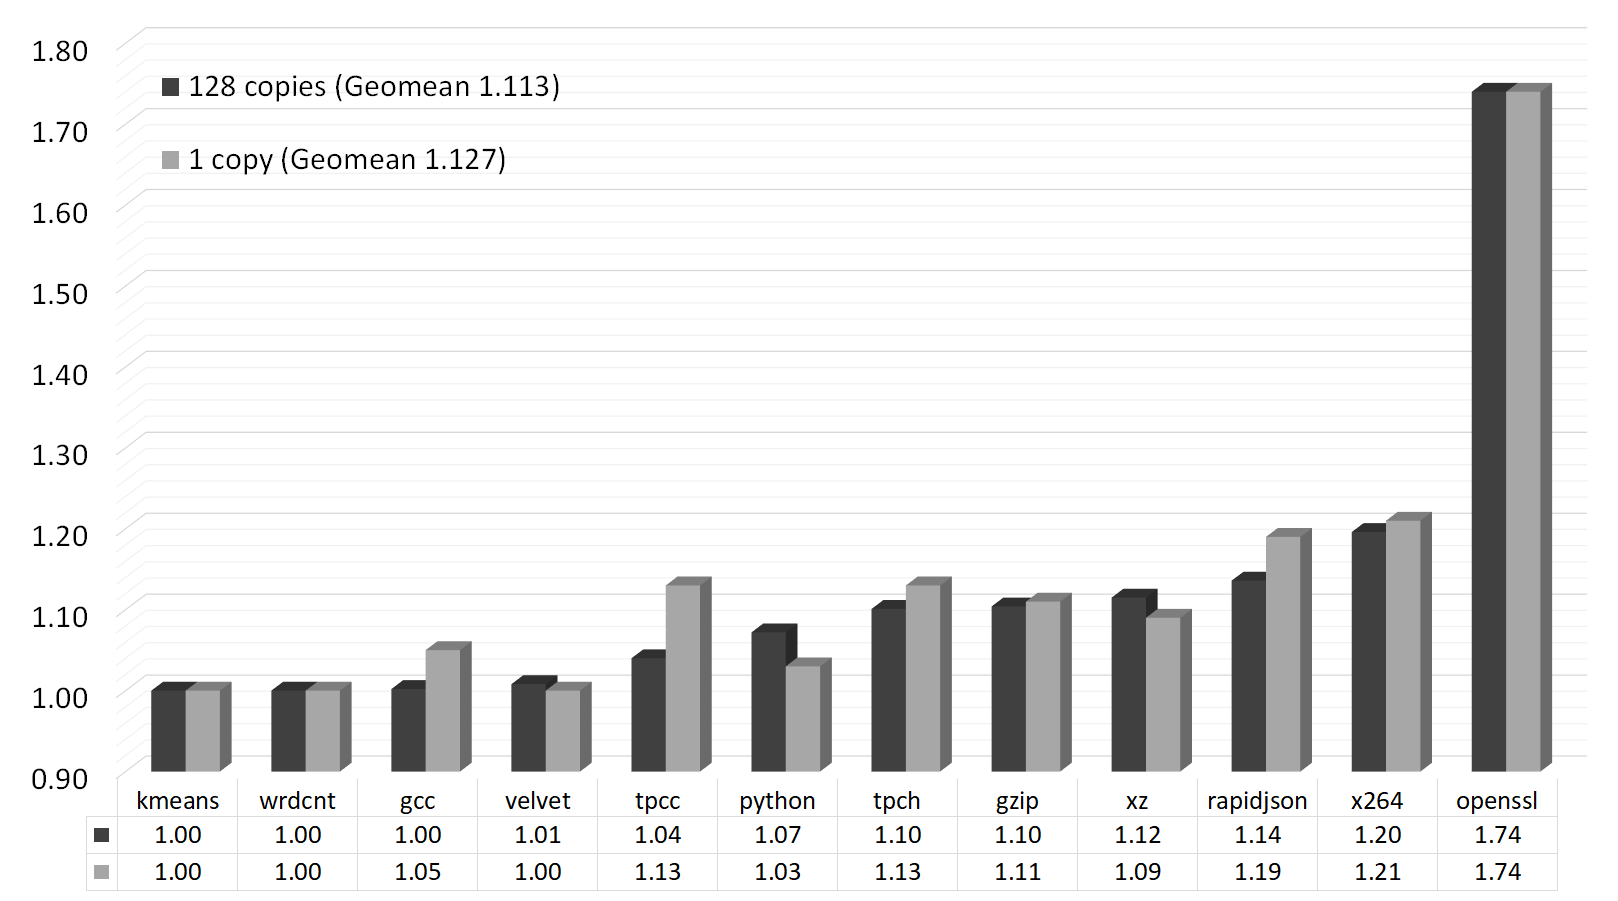
\includegraphics[scale=0.25]{PNG/speedup_combined3.png}
  	}
  	\caption{Результаты замеров производительности на тестах  пакета CPUBench int.}\label{fig:spubench_int_speedup}
  \end{figure}
  
  \begin{figure}[ht]
  	\centerfloat{
  		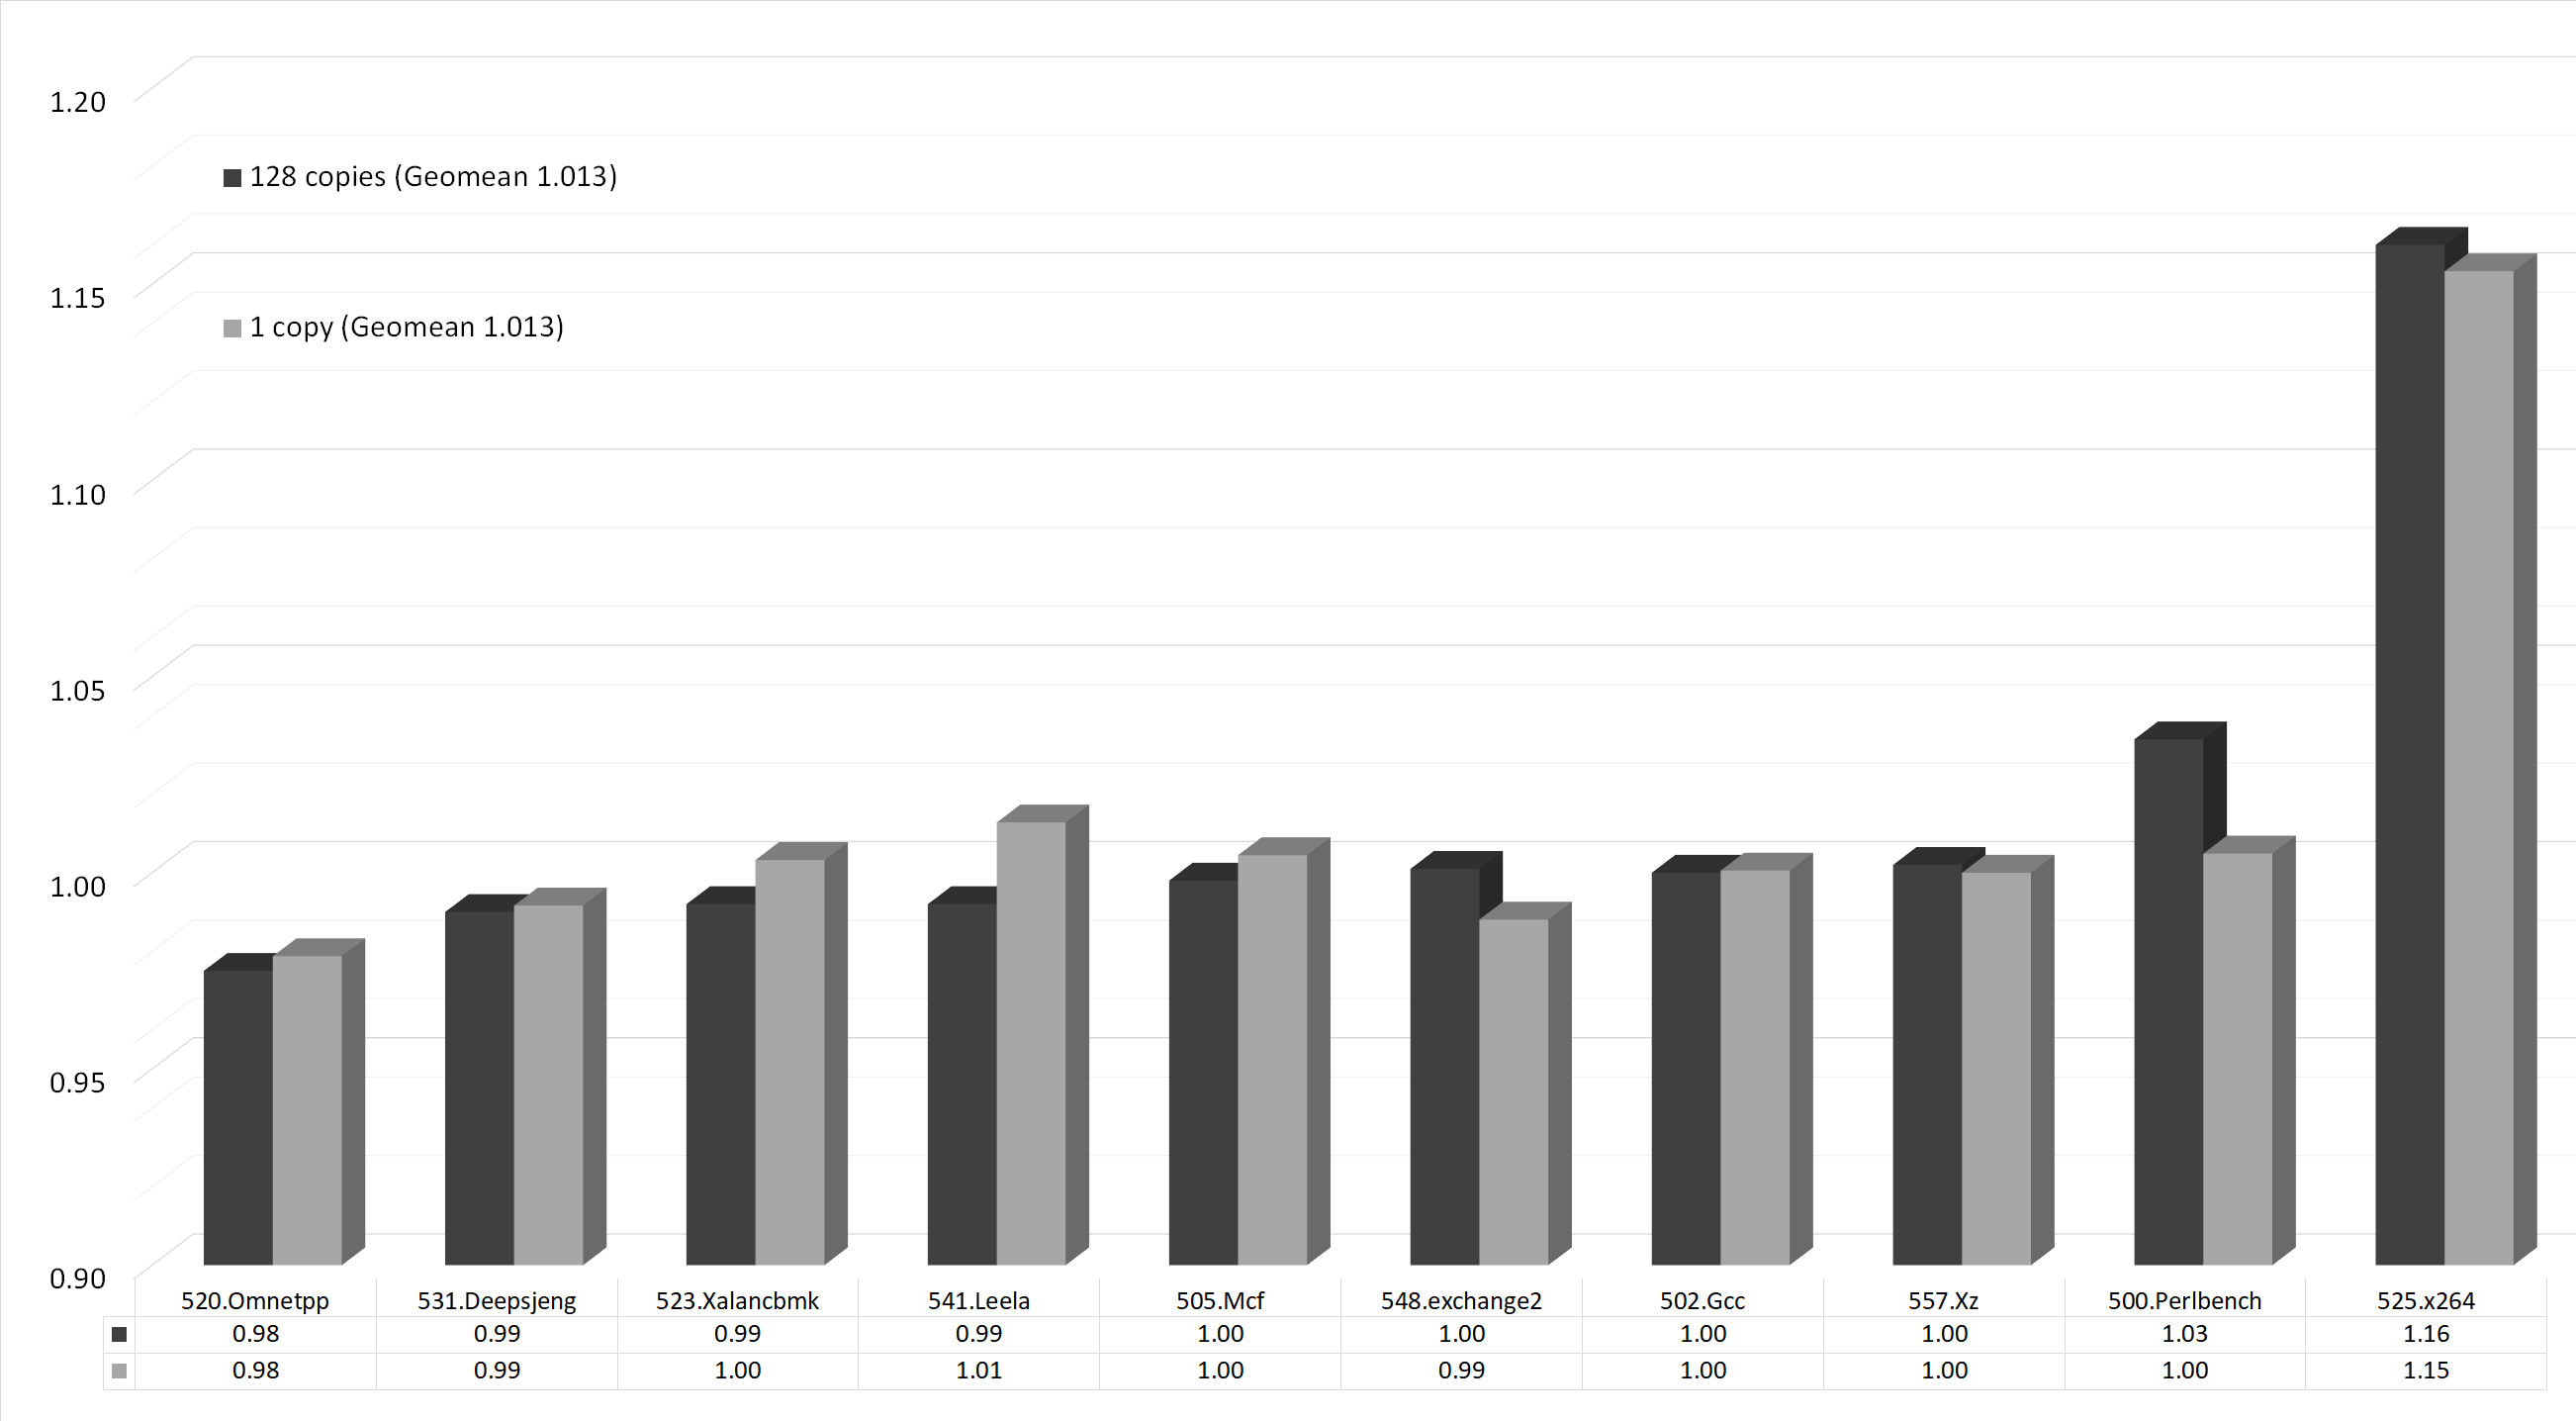
\includegraphics[scale=0.15]{PNG/spec_speedup.png}
  	}
  	\caption{Результаты замеров производительности на тестах  пакета SpecCPU int}\label{fig:spec_int_speedup}
  \end{figure}
  
%Можно сослаться на свои работы в автореферате. Для этого в файле
%\verb!Synopsis/setup.tex! необходимо присвоить положительное значение
%счётчику \verb!\setcounter{usefootcite}{1}!. В таком случае ссылки на
%работы других авторов будут подстрочными.
%Изложенные в третьей главе результаты опубликованы в~\cite{vakbib1, vakbib2}.
%Использование подстрочных ссылок внутри таблиц может вызывать проблемы.%

\FloatBarrier
\pdfbookmark{Заключение}{conclusion}                                  % Закладка pdf
В \underline{\textbf{заключении}} приведены основные результаты работы, которые заключаются в следующем:

\begin{enumerate}
	\item На основе анализа современных технологий оптимизации приложений были выдвинуты гипотезы и направления исследования для последующей оптимизации приложений с учетом недостатков целевой архитектуры.
	\item Предварительный анализ производительности с помощью таких приложений как \textbf{perf,radare2,GEM5} позволил доказать существование возможности  для оптимизаций целевых приложений на исследуемой микроархитектуре. 
	\item Для выполнения поставленных задач было создано семь дополнительных проходов в компиляторе GCC, а также предложено 5 улучшений существующих оптимизаций.
	\item Разработанное решение позволило продемонстрировать улучшение производительности в ~11 \% на целевых тестах пакета CPUBench int  с улучшением до 74 \% на отдельных приложениях. 
	\item Разработанное решение позволило продемонстрировать улучшение производительности в ~6 \% на целевых тестах пакета CPUBench fp  с улучшением до 40 \% на отдельных приложениях. Для тестов пакета CPUBench fp улучшение производительности на  одном ядре существенно отличается и составляет ~12 \% на целевых тестах.
\end{enumerate}

В заключение хочется выразить благодарность всем коллегам и студентам, без которых данная работа не была бы возможной. Отдельная благодарность и большая признательность выражается научном руководителю Доброву А.Д за поддержку и помощь на всем научном пути автора.
\pdfbookmark{Литература}{bibliography}                                % Закладка pdf
%При использовании пакета \verb!biblatex! список публикаций автора по теме
%диссертации формируется в разделе <<\publications>>\ файла
%\verb!common/characteristic.tex!  при помощи команды \verb!\nocite!

\ifdefmacro{\microtypesetup}{\microtypesetup{protrusion=false}}{} % не рекомендуется применять пакет микротипографики к автоматически генерируемому списку литературы
\urlstyle{rm}                               % ссылки URL обычным шрифтом
\ifnumequal{\value{bibliosel}}{0}{% Встроенная реализация с загрузкой файла через движок bibtex8
    \renewcommand{\bibname}{\large \bibtitleauthor}
    \nocite{*}
    \insertbiblioauthor           % Подключаем Bib-базы
    %\insertbiblioexternal   % !!! bibtex не умеет работать с несколькими библиографиями !!!
}{% Реализация пакетом biblatex через движок biber
    % Цитирования.
    %  * Порядок перечисления определяет порядок в библиографии (только внутри подраздела, если `\insertbiblioauthorgrouped`).
    %  * Если не соблюдать порядок "как для \printbibliography", нумерация в `\insertbiblioauthor` будет кривой.
    %  * Если цитировать каждый источник отдельной командой --- найти некоторые ошибки будет проще.
    %
    %% authorvak
    \nocite{vakbib1}%
    \nocite{vakbib2}%
    %
    %% authorwos
    \nocite{wosbib1}%
    \nocite{chernonog2023статический}%
    \nocite{chernonog2024widemem}%
    \nocite{confmiptlazy}%
    \nocite{confmiptml1}%
       
    %
    %% authorscopus
    \nocite{scbib1}%
    %
    %% authorpathent
    %\nocite{patbib1}%
    %
    %% authorprogram
    \nocite{progbib1}%
    %
    %% authorconf
    \nocite{confbib1}%
    \nocite{confbib2}%
    %
    %% authorother
    \nocite{bib1}%
    \nocite{bib2}%

    \ifnumgreater{\value{usefootcite}}{0}{
        \begin{refcontext}[labelprefix={}]
            \ifnum \value{bibgrouped}>0
                \insertbiblioauthorgrouped    % Вывод всех работ автора, сгруппированных по источникам
            \else
                \insertbiblioauthor      % Вывод всех работ автора
            \fi
        \end{refcontext}
    }{
        \ifnum \totvalue{citeexternal}>0
            \begin{refcontext}[labelprefix=A]
                \ifnum \value{bibgrouped}>0
                    \insertbiblioauthorgrouped    % Вывод всех работ автора, сгруппированных по источникам
                \else
                    \insertbiblioauthor      % Вывод всех работ автора
                \fi
            \end{refcontext}
        \else
            \ifnum \value{bibgrouped}>0
                \insertbiblioauthorgrouped    % Вывод всех работ автора, сгруппированных по источникам
            \else
                \insertbiblioauthor      % Вывод всех работ автора
            \fi
        \fi
        %  \insertbiblioauthorimportant  % Вывод наиболее значимых работ автора (определяется в файле characteristic во второй section)
        \begin{refcontext}[labelprefix={}]
            \insertbiblioexternal            % Вывод списка литературы, на которую ссылались в тексте автореферата
        \end{refcontext}
        % Невидимый библиографический список для подсчёта количества внешних публикаций
        % Используется, чтобы убрать приставку "А" у работ автора, если в автореферате нет
        % цитирований внешних источников.
        \printbibliography[heading=nobibheading, section=0, env=countexternal, keyword=biblioexternal, resetnumbers=true]%
    }
}
\ifdefmacro{\microtypesetup}{\microtypesetup{protrusion=true}}{}
\urlstyle{tt}                               % возвращаем установки шрифта ссылок URL
